\tikzset{every picture/.style={line width=0.75pt}} %set default line width to 0.75pt        

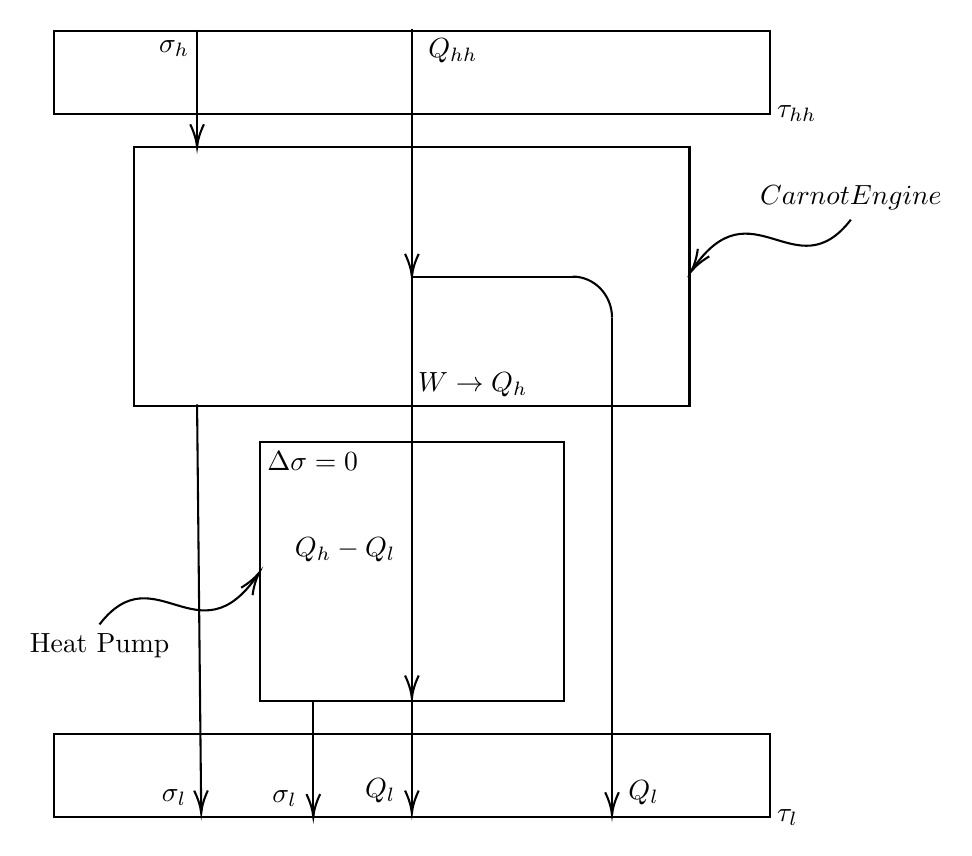
\begin{tikzpicture}[x=0.75pt,y=0.75pt,yscale=-1,xscale=1]
%uncomment if require: \path (0,444); %set diagram left start at 0, and has height of 444

%Shape: Rectangle [id:dp10170211024317433] 
\draw   (147,21) -- (492,21) -- (492,61) -- (147,61) -- cycle ;
%Shape: Rectangle [id:dp4544811596066871] 
\draw   (147,360) -- (492,360) -- (492,400) -- (147,400) -- cycle ;
%Shape: Rectangle [id:dp3842791172068818] 
\draw   (185.75,76.88) -- (453.25,76.88) -- (453.25,201.96) -- (185.75,201.96) -- cycle ;
%Shape: Rectangle [id:dp8874129257814114] 
\draw   (246.38,219.04) -- (392.63,219.04) -- (392.63,344.12) -- (246.38,344.12) -- cycle ;
%Curve Lines [id:da12079388453509687] 
\draw    (531,112) .. controls (504.27,146.65) and (483.42,94.07) .. (454.87,135.71) ;
\draw [shift={(454,137)}, rotate = 303.39] [color={rgb, 255:red, 0; green, 0; blue, 0 }  ][line width=0.75]    (10.93,-3.29) .. controls (6.95,-1.4) and (3.31,-0.3) .. (0,0) .. controls (3.31,0.3) and (6.95,1.4) .. (10.93,3.29)   ;
%Straight Lines [id:da13771774514472246] 
\draw    (319.5,20) -- (319.5,137.42) ;
\draw [shift={(319.5,139.42)}, rotate = 270] [color={rgb, 255:red, 0; green, 0; blue, 0 }  ][line width=0.75]    (10.93,-3.29) .. controls (6.95,-1.4) and (3.31,-0.3) .. (0,0) .. controls (3.31,0.3) and (6.95,1.4) .. (10.93,3.29)   ;
%Straight Lines [id:da42095144155513076] 
\draw    (319.5,139.42) -- (319.5,340.58) ;
\draw [shift={(319.5,342.58)}, rotate = 270] [color={rgb, 255:red, 0; green, 0; blue, 0 }  ][line width=0.75]    (10.93,-3.29) .. controls (6.95,-1.4) and (3.31,-0.3) .. (0,0) .. controls (3.31,0.3) and (6.95,1.4) .. (10.93,3.29)   ;
%Straight Lines [id:da693914432473546] 
\draw    (415.92,159.42) -- (415.92,396.84) ;
\draw [shift={(415.92,398.84)}, rotate = 270] [color={rgb, 255:red, 0; green, 0; blue, 0 }  ][line width=0.75]    (10.93,-3.29) .. controls (6.95,-1.4) and (3.31,-0.3) .. (0,0) .. controls (3.31,0.3) and (6.95,1.4) .. (10.93,3.29)   ;
%Straight Lines [id:da18101276066233973] 
\draw    (397.92,139.42) -- (319.5,139.42) ;
%Straight Lines [id:da8566525074884959] 
\draw    (216,20.58) -- (216,75) ;
\draw [shift={(216,77)}, rotate = 270] [color={rgb, 255:red, 0; green, 0; blue, 0 }  ][line width=0.75]    (10.93,-3.29) .. controls (6.95,-1.4) and (3.31,-0.3) .. (0,0) .. controls (3.31,0.3) and (6.95,1.4) .. (10.93,3.29)   ;
%Straight Lines [id:da2421143339083962] 
\draw    (272,343.29) -- (272,397.71) ;
\draw [shift={(272,399.71)}, rotate = 270] [color={rgb, 255:red, 0; green, 0; blue, 0 }  ][line width=0.75]    (10.93,-3.29) .. controls (6.95,-1.4) and (3.31,-0.3) .. (0,0) .. controls (3.31,0.3) and (6.95,1.4) .. (10.93,3.29)   ;
%Straight Lines [id:da6170237872934388] 
\draw    (319.5,342.58) -- (319.5,396) ;
\draw [shift={(319.5,398)}, rotate = 270] [color={rgb, 255:red, 0; green, 0; blue, 0 }  ][line width=0.75]    (10.93,-3.29) .. controls (6.95,-1.4) and (3.31,-0.3) .. (0,0) .. controls (3.31,0.3) and (6.95,1.4) .. (10.93,3.29)   ;
%Shape: Arc [id:dp5226403073336301] 
\draw  [draw opacity=0] (396.94,139.42) .. controls (396.94,139.42) and (396.94,139.42) .. (396.94,139.42) .. controls (396.94,139.42) and (396.94,139.42) .. (396.94,139.42) .. controls (407.42,139.42) and (415.92,148.28) .. (415.92,159.21) -- (396.94,159.21) -- cycle ; \draw   (396.94,139.42) .. controls (396.94,139.42) and (396.94,139.42) .. (396.94,139.42) .. controls (396.94,139.42) and (396.94,139.42) .. (396.94,139.42) .. controls (407.42,139.42) and (415.92,148.28) .. (415.92,159.21) ;  
%Curve Lines [id:da04778616308795569] 
\draw    (169,307) .. controls (195.73,272.35) and (216.58,324.93) .. (245.13,283.29) ;
\draw [shift={(246,282)}, rotate = 123.39] [color={rgb, 255:red, 0; green, 0; blue, 0 }  ][line width=0.75]    (10.93,-3.29) .. controls (6.95,-1.4) and (3.31,-0.3) .. (0,0) .. controls (3.31,0.3) and (6.95,1.4) .. (10.93,3.29)   ;
%Straight Lines [id:da8681702403313141] 
\draw    (216,201) -- (217.98,396) ;
\draw [shift={(218,398)}, rotate = 269.42] [color={rgb, 255:red, 0; green, 0; blue, 0 }  ][line width=0.75]    (10.93,-3.29) .. controls (6.95,-1.4) and (3.31,-0.3) .. (0,0) .. controls (3.31,0.3) and (6.95,1.4) .. (10.93,3.29)   ;

% Text Node
\draw (213.75,24.28) node [anchor=north east] [inner sep=0.75pt]    {$\sigma _{h}$};
% Text Node
\draw (216.75,395.9) node [anchor=south east] [inner sep=0.75pt]    {$\sigma _{l} \ $};
% Text Node
\draw (321.5,23.4) node [anchor=north west][inner sep=0.75pt]    {$\ Q_{hh}$};
% Text Node
\draw (417.92,395.44) node [anchor=south west] [inner sep=0.75pt]    {$\ Q_{l}$};
% Text Node
\draw (321,198.71) node [anchor=south west] [inner sep=0.75pt]    {$W\rightarrow Q_{h}$};
% Text Node
\draw (270,396.31) node [anchor=south east] [inner sep=0.75pt]    {$\sigma _{l} \ $};
% Text Node
\draw (317.5,278.18) node [anchor=south east] [inner sep=0.75pt]    {$Q_{h} -Q_{l} \ $};
% Text Node
\draw (317.5,394.6) node [anchor=south east] [inner sep=0.75pt]    {$Q_{l} \ $};
% Text Node
\draw (248.38,222.44) node [anchor=north west][inner sep=0.75pt]    {$\Delta \sigma =0$};
% Text Node
\draw (531,108.6) node [anchor=south] [inner sep=0.75pt]    {$\text{Carnot Engine}$};
% Text Node
\draw (169,310) node [anchor=north] [inner sep=0.75pt]   [align=left] {Heat Pump};
% Text Node
\draw (494,61) node [anchor=west] [inner sep=0.75pt]    {$\tau _{hh}$};
% Text Node
\draw (494,400) node [anchor=west] [inner sep=0.75pt]    {$\tau _{l}$};


\end{tikzpicture}
